\chapter{Initializing Vulkan}

In this chapter we go through all the necessary steps to initialize a
Vulkan application.
We first create a Vulkan instance.
Then, we create a window and link it to our Vulkan instance creating a presentation
surface.
We determine what GPU will be used by our application and create a logical device
to interface with it.
Finally, we create a swapchain in order to interface with the presentation engine
of our operating system.

\section{Create Vulkan Instance}

To access any of the functionalities offered by Vulkan we first have to create a Vulkan
instance.
To do this we call vkCreateInstance.

\begin{minipage}{\linewidth}{\noindent}
    \lstinputlisting[
        language=C++,
        caption={Create Vulkan instance},
        label={lst::CreateInstance}
        ]{src/ChInitializingVulkan/CreateInstance.cpp}
\end{minipage}

\subsection{VkInstanceCreateInfo}

We use a VkInstanceCreateInfo struct to configure the Vulkan instance we are about
to create.

\begin{minipage}{\linewidth}{\noindent}
\lstinputlisting[
    language=C++,
    caption={VkInstanceCreateInfo initialization},
    label={lst::VkInstanceCreateInfo}
    ]{src/ChInitializingVulkan/VkInstanceCreateInfo.cpp}
\end{minipage}

\subsection{VkApplicationInfo}

We can see that the VkInstanceCreateInfo struct is not the only thing we need.
We have to specify a pointer to a VkApplicationInfo struct. Such struct describes
our Vulkan application.

\begin{minipage}{\linewidth}{\noindent}
    \lstinputlisting[
        language=C++,
        caption={VkApplicationInfo initialization},
        label={lst::VkApplicationInfo}
        ]{src/ChInitializingVulkan/VkApplicationInfo.cpp}
\end{minipage}

\subsection{Layers}

While we initialize our VkInstanceCreateInfo struct, we can specify the layers
that we want to enable.
The specified layers will be loaded after the Vulkan instance creation.

Layers are optional components that hook into Vulkan.
Layers can intercept, evaluate and modify existing Vulkan functions.
Layers are implemented as libraries and are loaded during instance creation.

If we want to enable error checking, we need to load a layer that
provides such functionality.
This kind of layer is know as validation layer.
Since validation layers cause overhead, we can
disable them when we build the application in release mode.

\begin{minipage}{\linewidth}{\noindent}
    \lstinputlisting[
        language=C++,
        caption={Enabling the Khronos validation layer},
        label={lst::ValidationLayer}
        ]{src/ChInitializingVulkan/ValidationLayer.cpp}
\end{minipage}

\subsubsection{Checking whether our layers are supported}

Before creating our Vulkan instance, we should check if the layers we require are
actually supported.
To do this we use vkEnumerateInstanceLayerProperties.
This function returns all the layers supported by our Vulkan installation.
If all the layers we require are present, then we can proceed to create our
Vulkan instance.

\subsection{Extensions}

While we initialize our VkInstanceCreateInfo struct, we can specify the instance
extensions that we want to enable.
The specified instance extensions will be loaded after creating our Vulkan instance.

Extensions are  additional features that Vulkan implementations may provide.
Extensions add new functions and structs to the API.
Extensions may also change some of the behavior of existing functions.
We can either enable extensions at an instance level or at a device level.

We can use an extension to provide a callback to handle the debug messages
generated by the validation layers.

\begin{minipage}{\linewidth}{\noindent}
    \lstinputlisting[
        language=C++,
        caption={Enabling an extention to handle validation layer debug messages},
        label={lst::DebugExtension}
        ]{src/ChInitializingVulkan/DebugExtension.cpp}
\end{minipage}

We specify one callback that handles messages generated by
instance creation and destruction.
We also specify another callback that handles all other API debug messages.

\begin{minipage}{\linewidth}{\noindent}
    \lstinputlisting[
        language=C++,
        caption={Setting up debug extension callbacks},
        label={lst::DebugExtensionCallbacks}
        ]{src/ChInitializingVulkan/DebugExtensionCallbacks.cpp}
\end{minipage}

The function that creates the VkDebugUtilsMessengerEXT object comes from the
extension we have enabled.
Because of this, we have to load it manually into our address space using
vkGetInstanceProcAddr.
An elegant way to solve this issue is to create a proxy function that handles
this matter for us.

\begin{minipage}{\linewidth}{\noindent}
    \lstinputlisting[
        language=C++,
        caption={Extension function proxy},
        label={lst::ExtensionFunctionProxy}
        ]{src/ChInitializingVulkan/ExtensionFunctionProxy.cpp}
\end{minipage}

\subsubsection{Checking whether our extensions are supported}

Before creating our Vulkan instance, we should check if the instance extensions
we require are actually supported.
To do this we use vkEnumerateInstanceExtensionProperties.
This function returns all the instance extensions that are supported by our
Vulkan installation.
If all the instance extensions we require are present, then we can proceed to
create our Vulkan instance.

\subsection{Vulkan Instance Cleanup}

To destroy our debug messenger we use vkDestroyDebugUtilsMessengerEXT.
This function must be manually loaded using vkGetInstanceProcAddr.
To destroy our Vulkan instance we use vkDestroyInstance.

\section{Open A Window}

After creating our Vulkan instance we open a window.
To do this we have two options.
We can use a cross platform library (SDL, GLFW) that will do all the heavy lifting
for us, so that we don't have to worry about directly interacting with the OS,
freeing us from the burden of knowing how the windowing API works.
We can also decide to not use a library and opening the window ourselves.
We will do the latter, since it's interesting to know how things work under the hood.

Since I'm on Windows, I'll be dealing with the Win32 API.
We won't go in depth about the specifics of this API since it's beyond our scope.

\subsection{Create Window Handle}

To create a handle to a window we use CreateWindowEx.
We use windowStyle and windowExtendedStyle variables to configure the look of
our window.

\begin{minipage}{\linewidth}{\noindent}
    \lstinputlisting[
        language=C++,
        caption={Creating a window handle using Win32 API},
        label={lst::CreateWindowEx}
        ]{src/ChInitializingVulkan/CreateWindowEx.cpp}
\end{minipage}

\subsection{Computing Window Dimensions}

Before creating our window, we need to compute its width and height.
This is due to the fact that a window comprises of a client area and a non client area.
We usually want our client area to be of a certain size, but CreateWindowEx takes
the whole window width and the whole window height as arguments.

\begin{figure}[ht]
    \centering
    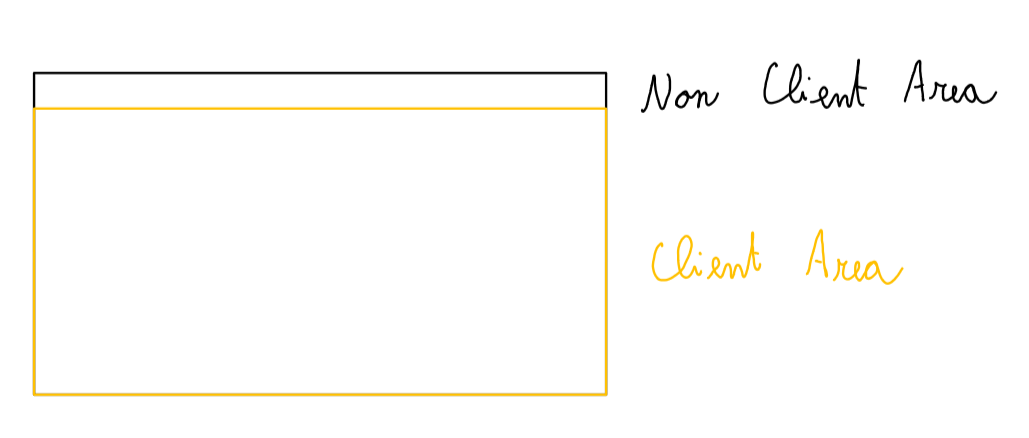
\includegraphics[scale=0.50]{images/ChInitializingVulkan/Win32Window.png}
    \caption{Anatomy of a Win32 Window}
    \label{fig::Win32Window}
\end{figure}

\begin{minipage}{\linewidth}{\noindent}
    \lstinputlisting[
        language=C++,
        caption={Compute window width and height},
        label={lst::AdjustWindowRectEx}
        ]{src/ChInitializingVulkan/AdjustWindowRectEx.cpp}
\end{minipage}

\subsection{Register Window Class}

Before creating our window, we need to register its window class.
To do this we use RegisterClassEx.
This function takes a pointer to a WNDCLASSEX struct.
This struct is used to configure our window class.

\begin{minipage}{\linewidth}{\noindent}
    \lstinputlisting[
        language=C++,
        caption={Register Window Class},
        label={lst::RegisterClassEx}
        ]{src/ChInitializingVulkan/RegisterClassEx.cpp}
\end{minipage}

\subsection{Window Procedure}

While filling in our WNDCLASSEX struct, we have to pass a window procedure.
This is a callback function used internally by the windowing API.
We use this function to handle the events that our window will receive during
the lifespan of our application.

The Win32 API also provides a default window procedure.
Our custom window procedure will call this default procedure when we don't want
to handle particular events ourselves.
When we receive a quit, close or destroy message we enqueue a quit message
into our message queue.

\begin{minipage}{\linewidth}{\noindent}
    \lstinputlisting[
        language=C++,
        caption={Window Procedure},
        label={lst::WindowProcedure}
        ]{src/ChInitializingVulkan/WindowProcedure.cpp}
\end{minipage}

\subsection{Process Window Messages}

In order for the user to be able to interact with our window, we need to handle
the window messages that are dispatched by the OS towards our window.
All these messages come from the application's message queue.

\begin{minipage}{\linewidth}{\noindent}
    \lstinputlisting[
        language=C++,
        caption={Process Window Messages},
        label={lst::ProcessWindowMessages}
        ]{src/ChInitializingVulkan/ProcessWindowMessages.cpp}
\end{minipage}

Here we iterate over all the window messages that we haven't handled.
If we find a quit message, then we exit our application.
All other messages will be dispatched to our window procedure.

\subsection{Window Cleanup}

When our application is shutting down, we destroy our window and unregister
its class.

\begin{minipage}{\linewidth}{\noindent}
    \lstinputlisting[
        language=C++,
        caption={Window Cleanup},
        label={lst::WindowCleanup}
        ]{src/ChInitializingVulkan/WindowCleanup.cpp}
\end{minipage}

\section{Create A Presentation Surface}

We must link our newly created window to our Vulkan instance.
To do this we create a presentation (or window) surface.
This operation is platform specific.
Since we are using Windows, in order to create our presentation surface we
use vkCreateWin32SurfaceKHR.

\begin{minipage}{\linewidth}{\noindent}
    \lstinputlisting[
        language=C++,
        caption={Create Presentation Surface},
        label={lst::CreatePresentationSurface}
        ]{src/ChInitializingVulkan/CreatePresentationSurface.cpp}
\end{minipage}

\subsection{VkWin32SurfaceCreateInfoKHR}

We use a VkWin32SurfaceCreateInfoKHR struct to configure the presentation
surface we are about to create.

\begin{minipage}{\linewidth}{\noindent}
    \lstinputlisting[
        language=C++,
        caption={Filling in a VkWin32SurfaceCreateInfoKHR struct},
        label={lst::VkWin32SurfaceCreateInfoKHR}
        ]{src/ChInitializingVulkan/VkWin32SurfaceCreateInfoKHR.cpp}
\end{minipage}

\subsection{Required Instance Extensions}

Vulkan, being cross platform, cannot interact directly with the OS windowing system.
To do this we use extensions.

The first extension that we enable is the instance level KHR surface extension.
This extension exposes a VkSurfaceKHR object that represents a surface to present
rendered images to.
This surface will be backed by the window we have created.

The second extension we enable is platform specific and is needed
to create our VkSurfaceKHR object.
In our case, since we are using Windows, we enable the instance level KHR win32
surface extension.

\begin{minipage}{\linewidth}{\noindent}
    \lstinputlisting[
        language=C++,
        caption={Presentation Surface Extensions},
        label={lst::PresentationSurfaceExtensions}
        ]{src/ChInitializingVulkan/PresentationSurfaceExtensions.cpp}
\end{minipage}

Notice the define preprocessor directive right before including our Vulkan header.
We do this to access our native platform functions.

\subsection{Presentation Surface Cleanup}

To destroy our presentation surface we use vkDestroySurfaceKHR.

\section{Pick A Physical Device}

Now that we have a Vulkan instance and a presentation surface, we select
a physical device (a GPU) that supports the features we need.
The selected GPU will be the one that will be used by our application.

\subsection{Listing Available Physical Devices}

We first get a list of all the physical devices that are available on the
system.
To do this we use vkEnumeratePhysicalDevices.
These physical devices can either be integrated or dedicated GPUs.

\subsection{Finding A Suitable Physical Device}

Now that we have a list of all the physical devices, we can select one of them.
We could, for example, automatically pick the first one without doing any kind
of checking.
This approach is doable if we don't have any particular requirement for our
physical devices.

Usually we have a set of specific physical device features that are mandatory
for our application to run.
Hence, in our list, some physical devices will be suitable for our application, while
others won't.

The approach we take here is to iterate through the list of all physical devices and
pick the first one that is suitable for our application.
One question still remains: how can we tell whether a physical device is suitable or not?

\subsubsection{Support Grpahics Operations}

To check if our physical device supports graphics operations we list all
the queue families of our physical device.
To do this we use vkGetPhysicalDeviceQueueFamilyProperties.
Then we check if at least one queue family supports graphics operations.

\begin{minipage}{\linewidth}{\noindent}
    \lstinputlisting[
        language=C++,
        caption={Check for graphics operations support},
        label={lst::SupportGraphicsOperations}
        ]{src/ChInitializingVulkan/SupportGraphicsOperations.cpp}
\end{minipage}

\subsubsection{Support Present Operations}

To check if our physical device supports present operations we list all
the queue families of our physical device.
To do this we use vkGetPhysicalDeviceQueueFamilyProperties.
Then we check if at least one queue family supports present operations.

\begin{minipage}{\linewidth}{\noindent}
    \lstinputlisting[
        language=C++,
        caption={Check for present operations support},
        label={lst::SupportPresentOperations}
        ]{src/ChInitializingVulkan/SupportPresentOperations.cpp}
\end{minipage}

\subsubsection{Support Presentation To A Surface}

Not only our physical device must support present operations.
It must also be able to present images to the screen.
Image presentation is tied to the window and consequently to the surface
associated with it.
For this reason, image presentation to the screen is not part of Vulkan.
We have to enable the KHR swapchain device extension to support such operation.
We need this particular extension because image presentation to a surface is
achieved using a swapchain.

\begin{minipage}{\linewidth}{\noindent}
    \lstinputlisting[
        language=C++,
        caption={Device extension for image presentation to the screen},
        label={lst::DeviceExtensions}
        ]{src/ChInitializingVulkan/DeviceExtensions.cpp}
\end{minipage}

As we have seen earlier, before enabling an extension, we should check for its
support.
To check whether our physical device supports one or more device extensions we use
vkEnumerateDeviceExtensionProperties.
This function returns a list of all the extensions supported by our physical device.
Then, we simply check whether all the extensions we require are present in the list.

\subsubsection{Support A Present Mode}

Checking if a swapchain is supported is not sufficient.
Even if it's supported, it may not be compatible with our presentation surface.
We need to check whether our physical device supports at least one present mode
for our presentation surface.
We can do this using vkGetPhysicalDeviceSurfacePresentModesKHR.
This functions returns a list of present modes supported by our physical device
that are compatible with our presentation surface.
If there is at least one present mode in the list, then we are good to go.

\section{Create A Logical Device}

To interact with the physical device we have selected we need to create
a logical device.

\begin{minipage}{\linewidth}{\noindent}
    \lstinputlisting[
        language=C++,
        caption={Create a logical device},
        label={lst::CreateDevice}
        ]{src/ChInitializingVulkan/CreateDevice.cpp}
\end{minipage}

\subsection{VkDeviceCreateInfo}

We use a VkDeviceCreateInfo struct to configure the device we are about to
create.

During physical device picking, we saved two queue family indices.
The first for a queue family that supports graphics operations.
The second for a queue family that supports present operations.
The way we populate our VkDeviceCreateInfo struct is different based on whether
these two indices are equal or not.
If our graphics and present queue families are the same, we tell our device that
we want to create a single queue.
Otherwise, we tell our device that we want to create two queues, one from our
graphics queue family, and the other from our present queue family.

\begin{minipage}{\linewidth}{\noindent}
    \lstinputlisting[
        language=C++,
        caption={Create info struct when queue families are the same},
        label={lst::VkDeviceCreateInfoSameQueueFamily}
        ]{src/ChInitializingVulkan/VkDeviceCreateInfoSameQueueFamily.cpp}
\end{minipage}

\begin{minipage}{\linewidth}{\noindent}
    \lstinputlisting[
        language=C++,
        caption={Create info struct when queue families are different},
        label={lst::VkDeviceCreateInfoDifferentQueueFamily}
        ]{src/ChInitializingVulkan/VkDeviceCreateInfoDifferentQueueFamily.cpp}
\end{minipage}

\subsection{Retrieve Queue Handles}

After creating our logical device, we retrieve the handles to the
queues we created.

\begin{minipage}{\linewidth}{\noindent}
    \lstinputlisting[
        language=C++,
        caption={Retrieve queue handles},
        label={lst::RetrieveQueueHandles}
        ]{src/ChInitializingVulkan/RetrieveQueueHandles.cpp}
\end{minipage}

\subsection{Cleanup}

We use vkDestroyDevice to destroy our logical device.

\section{Create A Swapchain}

After having created our logical device, we can create a swapchain object.
We need a swapchain to handle the logic for image presentation.
A swapchain creates and manages a set of images that can be presented to the screen.

\begin{minipage}{\linewidth}{\noindent}
    \lstinputlisting[
        language=C++,
        caption={Create a swapchain},
        label={lst::CreateSwapchain}
        ]{src/ChInitializingVulkan/CreateSwapchain.cpp}
\end{minipage}

\subsection{VkSwapchainCreateInfoKHR}

We use a VkSwapchainCreateInfoKHR struct to configure the swapchain we are
about to create.

\begin{minipage}{\linewidth}{\noindent}
    \lstinputlisting[
        language=C++,
        caption={Configure our swapchain},
        label={lst::VkSwapchainCreateInfoKHR}
        ]{src/ChInitializingVulkan/VkSwapchainCreateInfoKHR.cpp}
\end{minipage}

We have to additionally provide other data that depends on whether or not we use
the same queue for graphics and present operations.

\begin{minipage}{\linewidth}{\noindent}
    \lstinputlisting[
        language=C++,
        caption={Configure queue ownership over swapchain images},
        label={lst::VkSwapchainCreateInfoKHRQueues}
        ]{src/ChInitializingVulkan/VkSwapchainCreateInfoKHRQueues.cpp}
\end{minipage}

\subsection{Select The Minimum Swapchain Image Count}

Here we want to determine the minimum number of swapchain images to create.
We can do this by querying the surface capabilities with
vkGetPhysicalDeviceSurfaceCapabilitiesKHR.

\begin{minipage}{\linewidth}{\noindent}
    \lstinputlisting[
        language=C++,
        caption={Select swapchain image count},
        label={lst::SelectSwapchainImageCount}
        ]{src/ChInitializingVulkan/SelectSwapchainImageCount.cpp}
\end{minipage}

Here we would like to use one more image than the bare minimum.
This is due to the fact that, if we use the bare minimum number of images,
we may have to wait for the driver to complete internal operations before
we can acquire another swapchain image to render to.

Here we also have to be aware of the fact that there can be a maximum number of
swapchain images we can require.
Thus, we must be careful to cap the number of images that
we request to the nominal maximum.

\subsection{Select The Swapchain Image Format}

We must specify a proper format for our swapchain images.
To do this, we first query for all image formats that are supported by our
surface.
We can do this using vkGetPhysicalDeviceSurfaceFormatsKHR.

Once we have a list of valid formats we could either pick one randomly or
try to pick the one that we consider the best.

\begin{minipage}{\linewidth}{\noindent}
    \lstinputlisting[
        language=C++,
        caption={Select swapchain image format},
        label={lst::SelectSwapchainImageFormat}
        ]{src/ChInitializingVulkan/SelectSwapchainImageFormat.cpp}
\end{minipage}

We would like to use SRGB color space, with 32 bit RGBA format.

\subsection{Select The Swapchain Image Extent}

We must specify the resolution for our swapchain images.
This will almost always be equal to the resolution of our window.
Some windowing systems allow us to differ, indicating that the current
width and height are the maximum value of a an unsigned 32 bits integer.
In this scenario, we have to pick the resolution that best matches the window
within the bounds specified by our surface capabilities.

\begin{minipage}{\linewidth}{\noindent}
    \lstinputlisting[
        language=C++,
        caption={Select swapchain image extent},
        label={lst::SelectSwapchainImageExtent}
        ]{src/ChInitializingVulkan/SelectSwapchainImageExtent.cpp}
\end{minipage}

\subsection{Select The Swapchain Presentation Mode}

A presentation mode tells the conditions for showing our swapchain images to
the screen.

We start by listing all the presentation modes that our physical device supports
for presenting images to our surface.
We can do this using vkGetPhysicalDeviceSurfacePresentModesKHR.
We already did this while selecting our physical device.
After that, we check whether the mailbox presentation mode is supported.
We would like to use this present mode because it doesn't suffer from
tearing and it's not locked to the screen refresh rate.
If it's present we are good to go.
Otherwise we select the presentation mode that is guaranteed to be always supported:
\texttt{VK\_PRESENT\_MODE\_FIFO\_KHR}.

\begin{minipage}{\linewidth}{\noindent}
    \lstinputlisting[
        language=C++,
        caption={Select swapchain present mode},
        label={lst::SelectSwapchainPresentMode}
        ]{src/ChInitializingVulkan/SelectSwapchainPresentMode.cpp}
\end{minipage}

\subsection{Retrieve The Swapchain Images}

Now that we have created a swapchain we can retrieve the handles to the images
in it.
We use these images during rendering.
We can do this using vkGetSwapchainImagesKHR;

\subsection{Create Swapchain Image Views}

Vulkan doesn't allow us to use images directly.
Before using an image, we first have to create a view on it.
This also applies to our swapchain images.
Thus, for every image in the swapchain, we must create a corresponding
image view for it.

\begin{minipage}{\linewidth}{\noindent}
    \lstinputlisting[
        language=C++,
        caption={Create swapchain image views},
        label={lst::CreateSwapchainImageViews}
        ]{src/ChInitializingVulkan/CreateSwapchainImageViews.cpp}
\end{minipage}

\subsection{Cleanup}

We first have to destroy the swapchain image views using vkDestroyImageView.
We then destroy the swapchain itself using vkDestroySwapchainKHR.
The swapchain images will be automatically destroyed when we destroy our
swapchain.

\section{Our Application So Far}

Here we can see how all the parts we presented in this chapter fit together
to form our application.

\begin{minipage}{\linewidth}{\noindent}
    \lstinputlisting[
        language=C++,
        caption={Structure of our application},
        label={lst::Application}
        ]{src/ChInitializingVulkan/Application.cpp}
\end{minipage}
